\documentclass[a4paper,oneside,11pt,leqno]{article}

\usepackage[spanish,es-tabla]{babel}

\usepackage{graphicx}
\usepackage{booktabs}
\usepackage{amsmath}

\textwidth = 16truecm 
\textheight = 25truecm
\oddsidemargin =-20pt
\evensidemargin = 5pt
\topmargin=-2truecm

\setlength{\parskip}{\baselineskip}%
\begin{document}
	
	\section{Resultados CC}
	\label{sec:results_cc}
	
	El análisis estadístico se hizo entre 20 modelos (poblaciones) con 100 muestras emparejadas.
	
	El nivel de significancia para los test globales (\textit{family-wise}) es de $\alpha$=0.050.
	
	Rechazamos la hipótesis nula de que la población es normal para el modelo PLS + SVC (p=0.002). Por lo tanto asumimos no que todas las poblaciones son normales.
	
	Dado que tenemos más de dos poblaciones y que al menos una de ella no es normal, usamos el test no paramétrico de Friedman como test \textit{omnibus} para determinar si hay alguna diferencia significativa entre las medianas de las poblaciones. Utilizamos el test de Nemenyi como \textit{post-hoc} para saber que diferencias son significativas. Mostramos, en la tabla \ref{tab:stat_results_cc}, la mediana $(MD)$, la desviación absoluta sobre a la mediana $(MAD)$, y el ranking medio $(MR)$ de cada modelo a partir de todas las muestras. Consideraremos significativas la diferencias entre modelos si la diferencia entre rankings medios es mayor que la distancia crítica de $CD=2.965$ dada por el test de Nemenyi.

	Rechazamos la hipótesis nula $(p=6.26\times 10^{-58})$ del test de Friedman de que no hay diferencia entre las medidas de tendencia central de los modelos. Por lo que asumimos que hay una diferencia estadísticamente significativa entre las medianas de las poblaciones.
	
	\begin{table}[h]
		\centering
		\begin{tabular}{lrrllll}
			\toprule
			{} &     MR &   MED &   MAD &              CI & $\gamma$ &   Magnitude \\
			\midrule
			PCA + KNNSScaler   & 14.385 & 0.510 & 0.035 &  [0.493, 0.548] &     0.000 &  negligible \\
			PLS + KNNSScaler   & 13.690 & 0.520 & 0.036 &  [0.490, 0.556] &    -0.187 &  negligible \\
			mRMR + KNN         & 12.660 & 0.532 & 0.031 &  [0.510, 0.560] &    -0.437 &       small \\
			whole + SVC        & 12.525 & 0.533 & 0.033 &  [0.508, 0.562] &    -0.442 &       small \\
			PLS + KNN          & 12.380 & 0.522 & 0.036 &  [0.504, 0.562] &    -0.221 &       small \\
			PCA + SVC          & 12.155 & 0.535 & 0.041 &  [0.506, 0.571] &    -0.435 &       small \\
			mRMR + KNNSScaler  & 12.120 & 0.535 & 0.029 &  [0.514, 0.563] &    -0.508 &      medium \\
			PLS + SVC          & 11.370 & 0.548 & 0.028 &  [0.517, 0.568] &    -0.808 &       large \\
			PLS + SVCSScaler   & 11.170 & 0.543 & 0.035 &  [0.516, 0.573] &    -0.628 &      medium \\
			mRMR + SVCSScaler  & 11.095 & 0.548 & 0.032 &  [0.519, 0.576] &    -0.759 &      medium \\
			PCA + SVCSScaler   & 10.430 & 0.547 & 0.041 &  [0.520, 0.587] &    -0.657 &      medium \\
			whole + SVCSScaler & 10.365 & 0.547 & 0.031 &  [0.527, 0.578] &    -0.752 &      medium \\
			whole + KNN        & 10.245 & 0.550 & 0.036 &  [0.518, 0.582] &    -0.744 &      medium \\
			whole + KNNSScaler &  9.860 & 0.554 & 0.036 &  [0.523, 0.587] &    -0.821 &       large \\
			mRMR + SVC         &  9.820 & 0.552 & 0.033 &  [0.529, 0.585] &    -0.831 &       large \\
			PCA + KNN          &  9.125 & 0.561 & 0.032 &  [0.533, 0.585] &    -1.034 &       large \\
			PLS + LR           &  7.870 & 0.569 & 0.033 &  [0.545, 0.602] &    -1.152 &       large \\
			mRMR + LR          &  7.420 & 0.576 & 0.033 &  [0.547, 0.601] &    -1.298 &       large \\
			whole + LR         &  7.020 & 0.578 & 0.030 &  [0.555, 0.598] &    -1.396 &       large \\
			PCA + LR           &  4.295 & 0.604 & 0.032 &  [0.570, 0.623] &    -1.891 &       large \\
			\bottomrule
		\end{tabular}
		\caption{Comparativa del ROC AUC de los modelos con el dataset CC}
		\label{tab:stat_results_cc}
	\end{table}
	
	Basándonos en el test \textit{post-hoc} de Nemenyi, asumimos que no hay diferencia significativa dentro de los siguientes grupos:
	
	\begin{itemize}
		\item PCA + KNNSScaler, PLS + KNNSScaler, mRMR + KNN, whole + SVC, PLS + KNN, PCA + SVC, y mRMR + KNNSScaler
		
		\item PLS + KNNSScaler, mRMR + KNN, whole + SVC, PLS + KNN, PCA + SVC, mRMR + KNNSScaler, PLS + SVC, PLS + SVCSScaler, y mRMR + SVCSScaler
		
		\item mRMR + KNN, whole + SVC, PLS + KNN, PCA + SVC, mRMR + KNNSScaler, PLS + SVC, PLS + SVCSScaler, mRMR + SVCSScaler, PCA + SVCSScaler, whole + SVCSScaler, whole + KNN, whole + KNNSScaler, y mRMR + SVC
		
		\item PLS + SVC, PLS + SVCSScaler, mRMR + SVCSScaler, PCA + SVCSScaler, whole + SVCSScaler, whole + KNN, whole + KNNSScaler, mRMR + SVC, y PCA + KNN
		
		\item  PCA + SVCSScaler, whole + SVCSScaler, whole + KNN, whole + KNNSScaler, mRMR + SVC, PCA + KNN, y PLS + LR
		
		\item whole + SVCSScaler, whole + KNN, whole + KNNSScaler, mRMR + SVC, PCA + KNN, PLS + LR, y mRMR + LR
		
		\item  whole + KNNSScaler, mRMR + SVC, PCA + KNN, PLS + LR, mRMR + LR, y whole + LR
		
		\item whole + LR y PCA + LR
	\end{itemize}
	
	Todas las demás diferencias son significativas.
	
	\begin{figure}[h]
		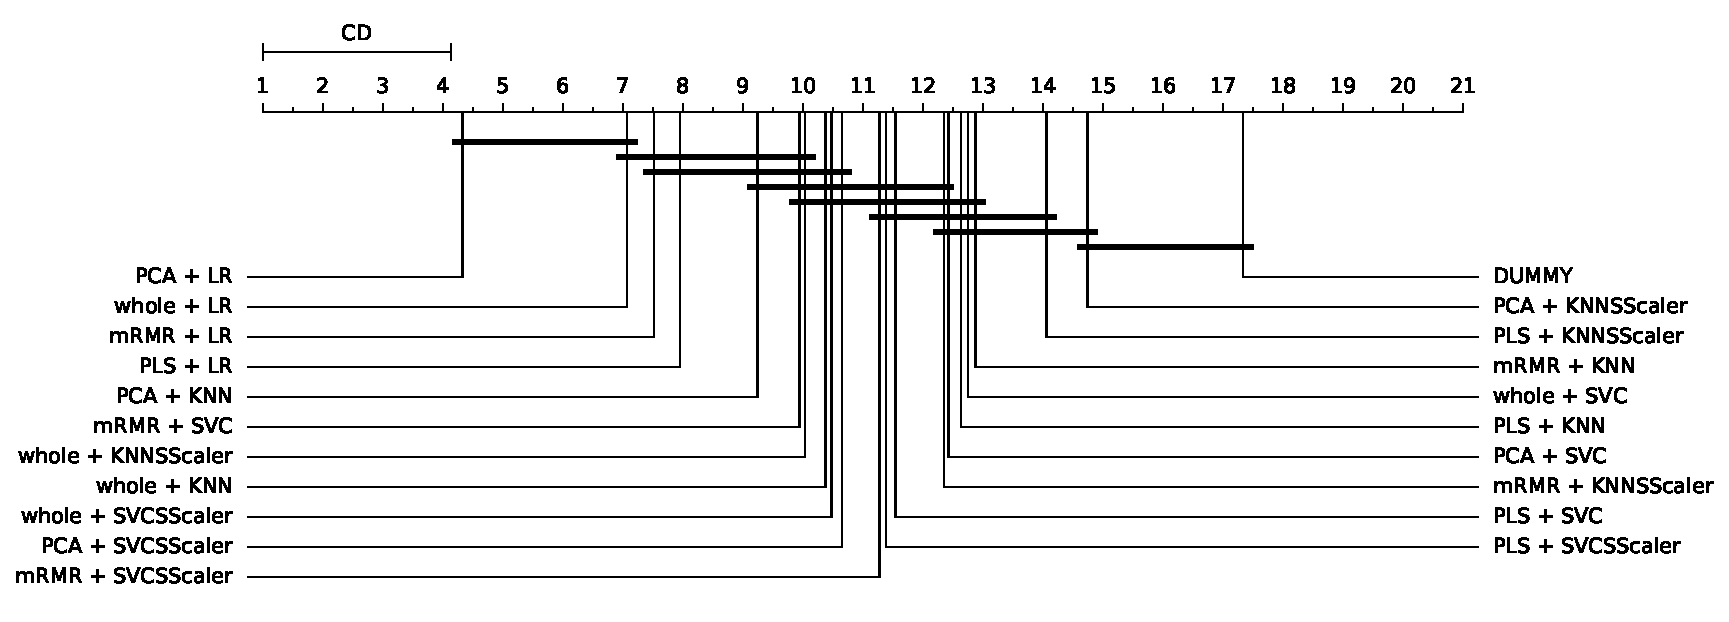
\includegraphics[width=\linewidth]{stat_results_cc.pdf}
		\caption{El diagrama CD representa los resultados del test Nemenyi para el ranking basado en el ROC AUC de ls modelos con el dataset CC. Las lineas horizontales representan diferencias no significativas}
		\label{fig:stats_fig_cc}
	\end{figure}

	\section{Resultados DCOR}
	\label{sec:results_dcor}
	
	El análisis estadístico se hizo entre 20 modelos (poblaciones) con 100 muestras emparejadas.
	
	El nivel de significancia para los test globales (\textit{family-wise}) es de $\alpha$=0.050.
	
	No hemos podido rechazar la hipótesis nula de que la población sea normal para ninguna población (mínimo $p=0.083$). Por lo tanto asumimos que las poblaciones son normales.
	
	Hemos aplicado el test Bartlett para evaluar la homogeneidad de los datos y rechazamos la hipótesis nula $(p=0.02)$ de que los datos son homocedásticos. Por lo que asumimos que los datos son heteroscedásticos.
	
	
	Dado que tenemos más de dos poblaciones, donde todas son normales pero heterocedásticas, usamos el test no paramétrico de Friedman como test \textit{omnibus} para determinar si hay alguna diferencia significativa entre las medias de las poblaciones. Utilizamos el test de Nemenyi como \textit{post-hoc} para saber que diferencias son significativas. Mostramos, en la tabla \ref{tab:stat_results_dcor}, la media $(M)$, la desviación estándar $(SD)$, y el ranking medio $(MR)$ de cada modelo a partir de todas las muestras. Consideraremos significativas la diferencias entre modelos si la diferencia entre rankings medios es mayor que la distancia crítica de $CD=2.965$ dada por el test de Nemenyi.

	Rechazamos la hipótesis nula $(p=5.88\times 10^{-85})$ del test de Friedman de que no hay diferencia entre las medidas de tendencia central de los modelos. Por lo que asumimos que hay una diferencia estadísticamente significativa entre las medianas de las poblaciones.
	
	\begin{table}[h]
		\centering
		\begin{tabular}{lrrrlll}
			\toprule
			{} &     MR &     M &    SD &              CI &    $d$ &   Magnitude \\
			\midrule
			PCA + SVC          & 13.260 & 0.465 & 0.045 &  [0.451, 0.479] &  0.000 &  negligible \\
			whole + SVCSScaler & 13.075 & 0.468 & 0.060 &  [0.450, 0.487] & -0.061 &  negligible \\
			whole + KNN        & 12.410 & 0.472 & 0.054 &  [0.455, 0.489] & -0.139 &  negligible \\
			PCA + SVCSScaler   & 12.395 & 0.474 & 0.044 &  [0.460, 0.487] & -0.193 &  negligible \\
			whole + KNNSScaler & 12.280 & 0.475 & 0.047 &  [0.460, 0.489] & -0.207 &       small \\
			whole + SVC        & 12.210 & 0.475 & 0.049 &  [0.460, 0.490] & -0.207 &       small \\
			PCA + KNN          & 11.535 & 0.479 & 0.050 &  [0.463, 0.494] & -0.287 &       small \\
			mRMR + KNNSScaler  & 10.885 & 0.486 & 0.050 &  [0.470, 0.501] & -0.437 &       small \\
			mRMR + SVCSScaler  & 10.870 & 0.483 & 0.053 &  [0.467, 0.500] & -0.370 &       small \\
			mRMR + KNN         & 10.705 & 0.487 & 0.056 &  [0.469, 0.504] & -0.424 &       small \\
			PCA + LR           & 10.510 & 0.488 & 0.040 &  [0.475, 0.500] & -0.526 &      medium \\
			mRMR + SVC         & 10.485 & 0.488 & 0.051 &  [0.472, 0.504] & -0.477 &       small \\
			PLS + SVC          &  9.440 & 0.495 & 0.055 &  [0.478, 0.512] & -0.596 &      medium \\
			PLS + KNN          &  9.320 & 0.499 & 0.052 &  [0.483, 0.515] & -0.689 &      medium \\
			PLS + KNNSScaler   &  9.185 & 0.500 & 0.052 &  [0.484, 0.516] & -0.720 &      medium \\
			whole + LR         &  8.865 & 0.501 & 0.044 &  [0.487, 0.515] & -0.804 &       large \\
			PCA + KNNSScaler   &  8.685 & 0.502 & 0.050 &  [0.486, 0.517] & -0.762 &      medium \\
			PLS + SVCSScaler   &  8.045 & 0.511 & 0.051 &  [0.495, 0.527] & -0.949 &       large \\
			mRMR + LR          &  7.985 & 0.509 & 0.046 &  [0.495, 0.523] & -0.960 &       large \\
			PLS + LR           &  7.855 & 0.512 & 0.051 &  [0.497, 0.528] & -0.982 &       large \\
			\bottomrule
		\end{tabular}
		\caption{Comparativa del ROC AUC de los modelos con el dataset DCOR}
		\label{tab:stat_results_dcor}
	\end{table}
	
	Basándonos en el test \textit{post-hoc} de Nemenyi, asumimos que no hay diferencia significativa dentro de los siguientes grupos:
	
	\begin{itemize}
		\item   PCA + SVC, whole + SVCSScaler, whole + KNN, PCA + SVCSScaler, whole + KNNSScaler, whole + SVC, PCA + KNN, mRMR + KNNSScaler, mRMR + SVCSScaler, mRMR + KNN, PCA + LR, y mRMR + SVC
		
		\item  PCA + SVCSScaler, whole + KNNSScaler, whole + SVC, PCA + KNN, mRMR + KNNSScaler, mRMR + SVCSScaler, mRMR + KNN, PCA + LR, mRMR + SVC, y PLS + SVC
		
		\item   whole + KNNSScaler, whole + SVC, PCA + KNN, mRMR + KNNSScaler, mRMR + SVCSScaler, mRMR + KNN, PCA + LR, mRMR + SVC, PLS + SVC, y PLS + KNN
		
		\item    PCA + KNN, mRMR + KNNSScaler, mRMR + SVCSScaler, mRMR + KNN, PCA + LR, mRMR + SVC, PLS + SVC, PLS + KNN, PLS + KNNSScaler, whole + LR, y PCA + KNNSScaler
		
		\item mRMR + KNNSScaler, mRMR + SVCSScaler, mRMR + KNN, PCA + LR, mRMR + SVC, PLS + SVC, PLS + KNN, PLS + KNNSScaler, whole + LR, PCA + KNNSScaler, PLS + SVCSScaler, y mRMR + LR
		
		\item  mRMR + KNN, PCA + LR, mRMR + SVC, PLS + SVC, PLS + KNN, PLS + KNNSScaler, whole + LR, PCA + KNNSScaler, PLS + SVCSScaler, mRMR + LR, y PLS + LR.
		
	\end{itemize}
	
	Todas las demás diferencias son significativas.
	
	
	\begin{figure}[h]
		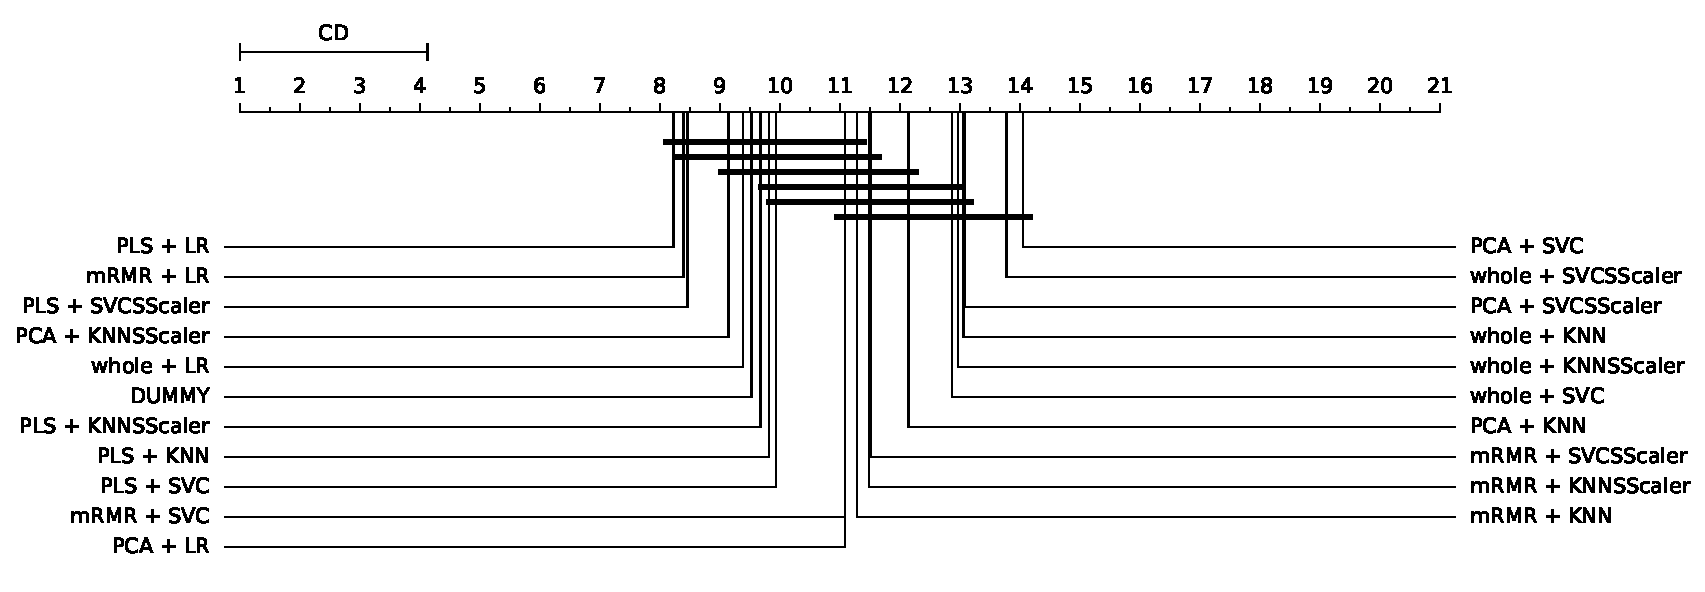
\includegraphics[width=\linewidth]{stat_results_dcor.pdf}
		\caption{El diagrama CD representa los resultados del test Nemenyi para el ranking basado en el ROC AUC de ls modelos con el dataset DCOR. Las lineas horizontales representan diferencias no significativas}
		\label{fig:stats_fig_dcor}
	\end{figure}
	
	\section{Resultados FFT}
	\label{sec:results_fft}
	
	El análisis estadístico se hizo entre 24 modelos (poblaciones) con 100 muestras emparejadas.
	
	El nivel de significancia para los test globales (\textit{family-wise}) es de $\alpha$=0.050.
	
	No hemos podido rechazar la hipótesis nula de que la población sea normal para ninguna población (mínimo $p=0.0028$). Por lo tanto asumimos que las poblaciones son normales.
	
	Dado que tenemos más de dos poblaciones, donde todas son normales pero heterocedásticas, usamos el test no paramétrico de Friedman como test \textit{omnibus} para determinar si hay alguna diferencia significativa entre las medias de las poblaciones. Utilizamos el test de Nemenyi como \textit{post-hoc} para saber que diferencias son significativas. Mostramos, en la tabla \ref{tab:stat_results_fft}, la media $(M)$, la desviación estándar $(SD)$, y el ranking medio $(MR)$ de cada modelo a partir de todas las muestras. Consideraremos significativas la diferencias entre modelos si la diferencia entre rankings medios es mayor que la distancia crítica de $CD=3.637$ dada por el test de Nemenyi.
	
	Rechazamos la hipótesis nula $(p=2.26\times 10^{-75})$ del test de Friedman de que no hay diferencia entre las medidas de tendencia central de los modelos. Por lo que asumimos que hay una diferencia estadísticamente significativa entre las medianas de las poblaciones.
	
	\begin{table}[h]
		\centering
		\begin{tabular}{lrrrlll}
			\toprule
			{} &     MR &     M &    SD &              CI &    $d$ &   Magnitude \\
			\midrule
			whole + SVC        & 19.180 & 0.500 & 0.000 &  [0.500, 0.500] &      - &       large \\
			PCA + SVC          & 17.600 & 0.504 & 0.049 &  [0.489, 0.520] & -0.130 &  negligible \\
			whole + LR         & 17.360 & 0.506 & 0.048 &  [0.491, 0.521] & -0.175 &  negligible \\
			PLS + KNNSScaler   & 15.690 & 0.520 & 0.049 &  [0.504, 0.535] & -0.568 &      medium \\
			mRMR + KNN         & 15.005 & 0.527 & 0.049 &  [0.511, 0.542] & -0.774 &      medium \\
			whole + KNN        & 14.700 & 0.528 & 0.047 &  [0.513, 0.543] & -0.849 &       large \\
			PCA + KNN          & 14.040 & 0.533 & 0.048 &  [0.518, 0.548] & -0.973 &       large \\
			PCA + KNNSScaler   & 13.870 & 0.534 & 0.047 &  [0.519, 0.549] & -1.037 &       large \\
			mRMR + KNNSScaler  & 13.810 & 0.535 & 0.050 &  [0.519, 0.551] & -0.993 &       large \\
			PLS + KNN          & 12.965 & 0.544 & 0.054 &  [0.527, 0.561] & -1.145 &       large \\
			PLS + SVCSScaler   & 12.870 & 0.542 & 0.054 &  [0.525, 0.559] & -1.121 &       large \\
			PCA + LRSScaler    & 12.825 & 0.545 & 0.057 &  [0.527, 0.563] & -1.115 &       large \\
			mRMR + SVC         & 12.450 & 0.545 & 0.051 &  [0.529, 0.561] & -1.242 &       large \\
			PCA + LR           & 11.715 & 0.553 & 0.055 &  [0.536, 0.571] & -1.375 &       large \\
			whole + KNNSScaler & 11.695 & 0.546 & 0.055 &  [0.529, 0.563] & -1.191 &       large \\
			PLS + SVC          & 11.200 & 0.554 & 0.058 &  [0.536, 0.573] & -1.328 &       large \\
			PLS + LRSScaler    & 10.690 & 0.559 & 0.054 &  [0.541, 0.576] & -1.524 &       large \\
			PLS + LR           & 10.645 & 0.556 & 0.053 &  [0.539, 0.573] & -1.503 &       large \\
			whole + LRSScaler  & 10.630 & 0.553 & 0.058 &  [0.535, 0.571] & -1.296 &       large \\
			PCA + SVCSScaler   & 10.470 & 0.555 & 0.053 &  [0.539, 0.572] & -1.481 &       large \\
			mRMR + SVCSScaler  &  8.450 & 0.574 & 0.050 &  [0.558, 0.589] & -2.075 &       large \\
			mRMR + LRSScaler   &  7.900 & 0.579 & 0.049 &  [0.563, 0.594] & -2.252 &       large \\
			mRMR + LR          &  7.380 & 0.583 & 0.046 &  [0.568, 0.597] & -2.539 &       large \\
			whole + SVCSScaler &  6.860 & 0.585 & 0.047 &  [0.570, 0.600] & -2.577 &       large \\
			\bottomrule
		\end{tabular}
		\caption{Comparativa del ROC AUC de los modelos con el dataset FFT}
		\label{tab:stat_results_fft}
	\end{table}
	
	Basándonos en el test \textit{post-hoc} de Nemenyi, asumimos que no hay diferencia significativa dentro de los siguientes grupos:
	
	\begin{itemize}
		\item whole + SVC, PCA + SVC, whole + LR, y PLS + KNNSScaler
		
		\item PCA + SVC, whole + LR, PLS + KNNSScaler, mRMR + KNN, whole + KNN, y PCA + KNN
		
		\item whole + LR, PLS + KNNSScaler, mRMR + KNN, whole + KNN, PCA + KNN, PCA + KNNSScaler, y mRMR + KNNSScaler
		
		\item PLS + KNNSScaler, mRMR + KNN, whole + KNN, PCA + KNN, PCA + KNNSScaler, mRMR + KNNSScaler, PLS + KNN, PLS + SVCSScaler, PCA + LRSScaler, y mRMR + SVC
		
		\item mRMR + KNN, whole + KNN, PCA + KNN, PCA + KNNSScaler, mRMR + KNNSScaler, PLS + KNN, PLS + SVCSScaler, PCA + LRSScaler, mRMR + SVC, PCA + LR, y whole + KNNSScaler
		
		\item whole + KNN, PCA + KNN, PCA + KNNSScaler, mRMR + KNNSScaler, PLS + KNN, PLS + SVCSScaler, PCA + LRSScaler, mRMR + SVC, PCA + LR, whole + KNNSScaler, y PLS + SVC
		
		\item PCA + KNN, PCA + KNNSScaler, mRMR + KNNSScaler, PLS + KNN, PLS + SVCSScaler, PCA + LRSScaler, mRMR + SVC, PCA + LR, whole + KNNSScaler, PLS + SVC, PLS + LRSScaler, PLS + LR, whole + LRSScaler, y PCA + SVCSScaler
		
		\item PCA + LR, whole + KNNSScaler, PLS + SVC, PLS + LRSScaler, PLS + LR, whole + LRSScaler, PCA + SVCSScaler, y mRMR + SVCSScaler
		
		\item PLS + SVC, PLS + LRSScaler, PLS + LR, whole + LRSScaler, PCA + SVCSScaler, mRMR + SVCSScaler, y mRMR + LRSScaler
		
		\item PLS + LRSScaler, PLS + LR, whole + LRSScaler, PCA + SVCSScaler, mRMR + SVCSScaler, mRMR + LRSScaler, y mRMR + LR
		
		\item PCA + SVCSScaler, mRMR + SVCSScaler, mRMR + LRSScaler, mRMR + LR, y whole + SVCSScaler
		
	\end{itemize}
	
	Todas las demás diferencias son significativas.
	
	
	\begin{figure}[h]
		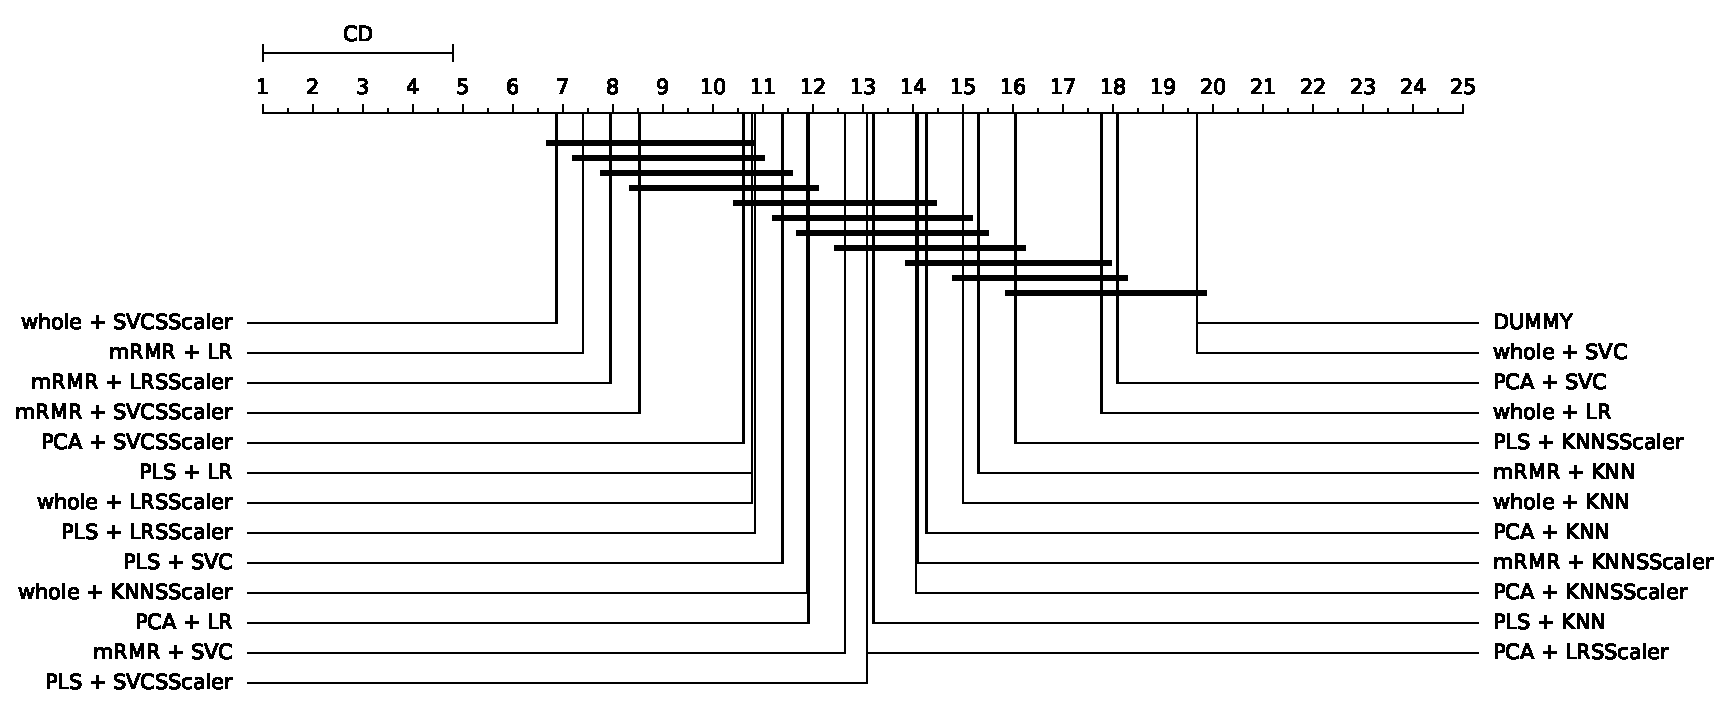
\includegraphics[width=\linewidth]{stat_results_fft.pdf}
		\caption{El diagrama CD representa los resultados del test Nemenyi para el ranking basado en el ROC AUC de ls modelos con el dataset DCOR. Las lineas horizontales representan diferencias no significativas}
		\label{fig:stats_fig_fft}
	\end{figure}

\end{document}